\chapter{Understanding F1Tenth ROS Control}

This chapter provides a detailed explanation of how the F1Tenth autonomous racing car interacts with ROS 2 using a simple wall following example written in Python.  We will dissect the code, explaining the purpose of each section and how it relates to the overall ROS 2 communication and control process.

\section{Code Overview}

The provided Python code implements a wall following algorithm for the F1Tenth car. It uses a Proportional-Integral-Derivative (PID) controller to maintain a desired distance from a wall.  The code interacts with the simulator through ROS 2 topics such as \ref{fig:ros}.

\subsection{ROS 2 Node and Topic Setup}

The code defines a ROS 2 node named \texttt{wall\_follow\_node}.  This node subscribes to the \texttt{/scan} topic, which publishes \texttt{LaserScan} messages containing LiDAR data, and publishes to the \texttt{/drive} topic, which accepts \texttt{AckermannDriveStamped} messages to control the car's steering and speed.

\begin{figure}
    \centering
    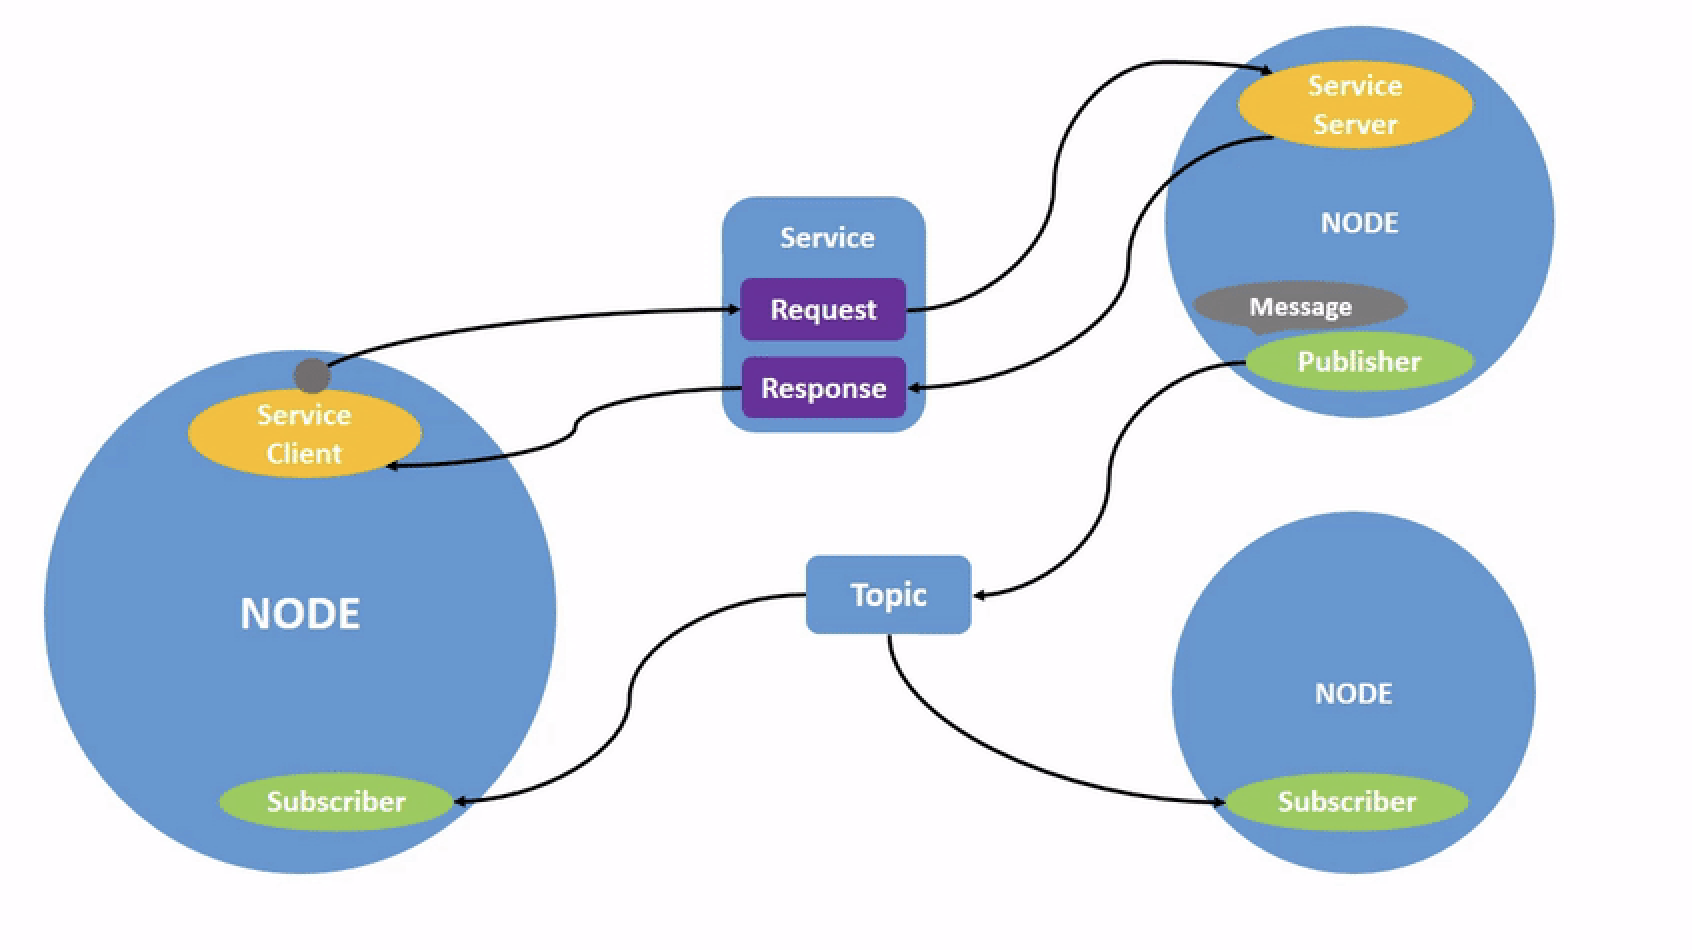
\includegraphics[scale=0.2]{ROS2}
    \caption{Basic ROS2 workflow}
    \label{fig:ros}
\end{figure}

\begin{verbatim}
lidarscan_topic = '/scan'
drive_topic = '/drive'

self.sub_scan = self.create_subscription(LaserScan, ...
self.pub_drive = self.create_publisher(AckermannDriveStamped, ...
\end{verbatim}

These lines of code set up the communication channels.  \texttt{self.create\_subscription} creates a subscriber that listens for \texttt{LaserScan} messages on the \texttt{/scan} topic and calls the \texttt{scan\_callback} function whenever a new message arrives.  \texttt{self.create\_publisher} creates a publisher that sends \texttt{AckermannDriveStamped} messages on the \texttt{/drive} topic to control the car.

\subsection{Helper Functions}

The code includes helper functions to process the LiDAR data and calculate the error.

\subsubsection{\texttt{get\_range(range\_data, angle)}}

This function takes the raw LiDAR data and an angle as input and returns the corresponding range measurement at that angle. It handles potential \texttt{NaN} (Not a Number) and \texttt{inf} (infinity) values in the LiDAR data.

\subsubsection{\texttt{get\_error(range\_data, dist)}}

This function calculates the error, which is the difference between the desired distance to the wall (\texttt{dist}) and the actual distance calculated from the LiDAR data.  It uses geometric calculations based on LiDAR readings at specific angles to estimate the distance to the wall.

\subsection{PID Control}

The \texttt{pid\_control} function implements the PID controller.  It takes the calculated error, desired velocity, time difference (\texttt{delta\_t}), and some additional LiDAR beam measurements as input.  It calculates the steering angle based on the PID gains (\texttt{kp}, \texttt{ki}, \texttt{kd}) and publishes the control command to the \texttt{/drive} topic.  The code also includes a simple obstacle avoidance mechanism based on the front LiDAR beam.

\begin{verbatim}
self.integral += self.ki * self.error * delta_t
angle = self.kp * self.error + np.clip(self.integral, -1, +1) ...

drive_msg.drive.speed = velocity
drive_msg.drive.steering_angle = angle
self.pub_drive.publish(drive_msg)
\end{verbatim}

This section calculates the PID output (steering angle) and publishes it along with the desired speed as an \texttt{AckermannDriveStamped} message.

\subsection{Scan Callback}

The \texttt{scan\_callback} function is the heart of the wall following algorithm.  It is called every time a new \texttt{LaserScan} message is received.  This function performs the following steps:

\begin{enumerate}
    \item Calculates the time elapsed since the last message.
    \item Calls \texttt{get\_error} to calculate the error.
    \item Calculates the desired car velocity based on the current heading angle.
    \item Calls \texttt{pid\_control} to calculate the steering angle and publish the drive message.
    \item Updates the previous time.
\end{enumerate}

\subsection{Main Function}

The \texttt{main} function initializes the ROS 2 node, creates the \texttt{WallFollow} object, and starts the ROS 2 event loop using \texttt{rclpy.spin()}.  This keeps the node alive and processes incoming messages. The final result of the program should look something like this: \ref{fig:struct}

\begin{figure}
    \centering
    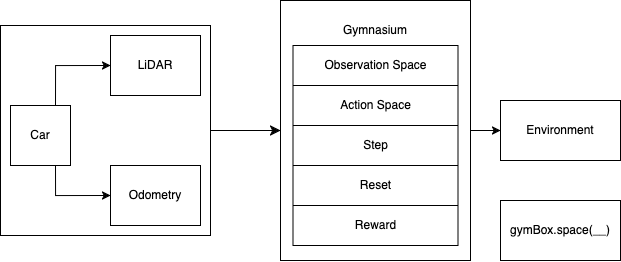
\includegraphics[scale=0.5]{structure}
    \caption{Structure of the program}
    \label{fig:struct}
\end{figure}

\section{ROS 2 Communication Flow}

The LiDAR sensor data is published on the \texttt{/scan} topic.  The \texttt{wall\_follow\_node} subscribes to this topic, processes the data, and publishes control commands on the \texttt{/drive} topic.  The F1Tenth car's actuators subscribe to the \texttt{/drive} topic and execute the commands.

This example demonstrates a basic ROS 2 node that interacts with sensor data and publishes control commands. It showcases the fundamental concepts of ROS 2 communication and provides a foundation for more complex autonomous driving algorithms.